%% Файл стиля для оформления дипломной работы

\documentclass[14pt,a4paper,oneside]{extarticle}

\usepackage[russian]{babel}	% Использование русского языка (работает расстановка переносов)
\usepackage[utf8]{inputenc}	% Кодировка utf8
\usepackage[T2A]{fontenc}	% Шрифт русский, Times New Roman
\usepackage{cmap} 		% Улучшенный поиск русских слов в полученном pdf-файле

\usepackage{indentfirst} 	% Включить отступ у первого абзаца

\usepackage{setspace}		% Полуторный интервал
\onehalfspacing

\usepackage{fancyhdr}		% Нумерация страниц в нижнем правом углу
\fancypagestyle{rightbottom} {
\renewcommand{\headrulewidth}{0pt}
	\fancyhead{}
	\fancyfoot{}
	\fancyfoot[R]{\thepage}
}
\pagestyle{rightbottom}

\renewcommand\contentsname{Содержание} % Переименовываем заголовок Содержания

\usepackage[a4paper, 			% Отступы с краев листа
	left=3.5cm, right=1.5cm, 
	top=2cm, bottom=2cm, 
	footskip=1.25cm]{geometry} 
	
% Заголовки разделов без нумерации
\newcommand{\anonsection}[1]{\section*{#1}\addcontentsline{toc}{section}{#1}}
\newcommand{\anonsubsection}[1]{\subsection*{#1}\addcontentsline{toc}{subsection}{#1}}
\newcommand{\anonsubsubsection}[1]{\subsubsection*{#1}\addcontentsline{toc}{subsubsection}{#1}}

% Точка в конце номаре раздела
\renewcommand{\theequation}{\thesection.\arabic{equation}}
\renewcommand{\thesubsubsection}{\arabic{section}.\arabic{subsection}.\arabic{subsubsection}.}
\renewcommand{\thesubsection}{\arabic{section}.\arabic{subsection}.}
\renewcommand{\thesection}{\arabic{section}.}

\setcounter{tocdepth}{3}	% Включать в оглавление заголовки до 3-го уровня включительно

\usepackage{graphicx} 		% Использование изображений
\graphicspath{{img/}}		% Путь к каталогу с изображениями

\newcommand{\pic}[1]{\ref{#1}} 	% Ссылка на изображение
\newcommand{\tab}[1]{\ref{#1}} 	% Ссылка на таблицу

\usepackage[tableposition=top]{caption}
\usepackage{subcaption}
\DeclareCaptionLabelFormat{gostfigure}{\textbf{Рис. #2.}}	% Подпись к рисунку
\DeclareCaptionLabelFormat{gosttable}{\textbf{Табл. #2.}}	% Подпись к таблице
\DeclareCaptionLabelSeparator{gost}{~ ~}
\captionsetup{labelsep=gost}
\captionsetup[figure]{labelformat=gostfigure}
\captionsetup[table]{labelformat=gosttable}
\renewcommand{\thesubfigure}{\asbuk{subfigure}}

\usepackage{multirow}		% Возможность объединения нескольких ячеек таблицы в одну

% Изменение оформления нумерации списка литературы
\makeatletter
\renewcommand{\@biblabel}[1]{#1.\hfil}
\makeatother
\bibliographystyle{utf8gost705u}	% Cтилевой файл для оформления по ГОСТу

\usepackage{listings}			% Для оформления исходного кода

\begin{document}
\thispagestyle{empty}
\begin{singlespacing}

\begin{center}
{\small МИНИСТЕРСТВО ОБРАЗОВАНИЯ И НАУКИ РОССИЙСКОЙ ФЕДЕРАЦИИ 	\\*
Федеральное государственное бюджетное образовательное учреждение \\*
высшего профессионального образования}							\\*
\textbf{«Южно-Уральский государственный университет» 			\\*
(национальный исследовательский университет) 					\\*
{\small Факультет Вычислительной математики и информатики 		\\*
Кафедра системного программирования}}
\end{center}

\vspace{60pt}

\begin{center}
\textbf{КУРСОВОЙ ПРОЕКТ} \\*
бакалавра направления 010400.62 "Информационные технологии" \\*
по дисциплине "Технологии анализа данных"
\end{center}

\vspace{24pt}

\begin{center}
\textbf{Разработка приложения интеллектуального анализа данных \\*
на платформе СУБД MySQL}
\end{center}

\vspace{24pt}

\begin{tabular}{p{0.5\linewidth}p{0.5\linewidth}}
&
Выполнил:			 		\par
студент группы ВМИ-456		\par
Е.М. Лукичева				\par
~							\par
~							\par
Проверил:					\par
М.Л. Цымблер					\par
Оценка: \makebox[1.0in]{\hrulefill}\par
Подпись:	 \makebox[1.0in]{\hrulefill}\par
Дата: \makebox[1.0in]{\hrulefill}\par
\\
\end{tabular}

\vfill

\begin{center}
Челябинск-2014
\end{center}

\end{singlespacing}

\tableofcontents		% Оглавление
\thispagestyle{fancy}

\section{Задание}
\subsection{Предметная область}
Компания занимается сборочным  производством и  продажей сложных устройств из деталей, закупаемых у поставщиков. Компания имеет два филиала, которые географически удалены друг от друг и имеютотличающуюся информационную структуру.\par
Аналитик компании выполняет подготовку  различных  оперативных  и аналитических  отчетов, целью которых  является увеличение эффективности деятельности компании в целом.\par
Необходимо  разработать программную систему анализа бизнес-данных для аналитика компании, которая выполняет следующие основные функции: интеграция  данных  из  филиалов  в  хранилище данных  компании, подготовка оперативных и аналитических отчетов.\par
Далее приведено описание сущностей предметной области. \par
При описании сущностей используются обозначения, указанные в \tab{semantic}.
\begin{table}[h]
	\caption{\space Обозначения атрибутов сущностей}
	\label{semantic}
	\begin{tabular}{|p{5cm}|p{10cm}|}
		\hline
		\textbf{Обозначение} & \textbf{Семантика}\\
		\hline
		* & Атрибут является первичным ключом сущности\\
		\hline
		\textasciicircum Сущность.Атрибут & Атрибут является внешним ключом и ссылается на указанный атрибут указанной сущности\\
		\hline
	\end{tabular}
\end{table}

В предметной области выделены сущности Поставщик, Деталь и Поставка. Описание сущности Поставщик представлено в табл. \tab{supplier}
\begin{table}[h]
	\caption{\space Атрибуты сущности Поставщик (S)}
	\label{supplier}
	\begin{tabular}{|p{0.4cm}|p{2.5cm}|p{1.5cm}|p{6.3cm}|p{3.2cm}|}
		\hline
		\textbf{№} & \textbf{Атрибут} & \textbf{Ключ} & \textbf{Семантика} & \textbf{Тип данных} \\
		\hline
		1. & SID & * & Уникальный код поставщика & INT \\
		\hline
		2. & SName &  & Имя поставщика & CHAR(20) \\
		\hline
		3. & SCity & & Город поставщика & CHAR(20) \\
		\hline
		4. & Address & & Почтовый адрес поставщика & CHAR(20) \\
		\hline
		5. & Risk & & Риск сотрудничества с поставщиком (низкий, средний, высокий) & (1, 2, 3) \\
		\hline
	\end{tabular}
\end{table}

Атрибуты сущности Деталь представлены в табл. \tab{part}.
\begin{table}[h]
	\caption{\space Атрибуты сущности Деталь (P)}
	\label{part}
	\begin{tabular}{|p{0.4cm}|p{2.5cm}|p{1.5cm}|p{6.3cm}|p{3.2cm}|}
		\hline
		\textbf{№} & \textbf{Атрибут} & \textbf{Ключ} & \textbf{Семантика} & \textbf{Тип данных} \\
		\hline
		1. & PID & * & Уникальный код детали & INT \\
		\hline
		2. & PName &  & Имя детали & CHAR(20) \\
		\hline
		3. & HTP & & Является ли деталь продуктом высоких технологий (High Technology Product) & BOOL \\
		\hline
		4. & Weight & & Вес детали в килограммах & FLOAT \\
		\hline
	\end{tabular}
\end{table}

Описание атрибутов сущности  Поставка представлено в табл. \tab{relation}.
\begin{table}[h]
	\caption{\space Атрибуты сущности Поставка (SP)}
	\label{relation}
	\begin{tabular}{|p{0.4cm}|p{2.5cm}|p{1.5cm}|p{6.3cm}|p{3.2cm}|}
		\hline
		\textbf{№} & \textbf{Атрибут} & \textbf{Ключ} & \textbf{Семантика} & \textbf{Тип данных} \\
		\hline
		1. & SPID & * & Уникальный код поставки & INT \\
		\hline
		2. & SID & \textasciicircum S.SID & Уникальный код поставщика & INT \\
		\hline
		3. & PID & \textasciicircum P.PID & Уникальный код детали & INT \\
		\hline
		4. & Qty & & Количество деталей в поставке & INT \\
		\hline
		5. & Price & & Цена за 1 шт. & FLOAT \\
		\hline
		6. & OrderDate & & Дата заказа поставки & DATE \\
		\hline
		7. & Period & & Срок доставки в днях & INT \\
		\hline
		8. & ShipDate & & Фактическая дата доставки & DATE \\
		\hline
	\end{tabular}
\end{table}

Данные  в  каждом из  филиалов  должны  подчиняться ограничениям целостности, 
перечисленным в табл. \tab{integrity}.Тем не менее,в филиалах не всегда 
осу-ществляется проверка целостности вводимых данных, вследствие чего в дан-ных 
возможны ошибки.
\begin{table}[h]
	\caption{\space Ограничения целостности}
	\label{integrity}
	\begin{tabular}{|p{4cm}|p{8cm}|}
		\hline
		\textbf{Сущность} & \textbf{Ограничение целостности} \\
		\hline
		\multirow{4}{*}{S} 	& SName NOT NULL \\
					& SCity NOT NULL \\
					& Address NOT NULL \\
					& (SName, Address, SCity) UNIQUE \\
		\hline
		\multirow{3}{*}{P}	& PName NOT NULL\\
					& Weight > 0\\
					& HTP in (0, 1) \\
					& (PName, Weight) UNIQUE \\
		\hline
		\multirow{5}{*}{SP}	& OrderDate NOT NULL \\
					& Qty > 0 \\
					& Price > 0 \\
					& Period >= 0 \\
					& OrderDate <= ShipDate \\
		\hline
		S, P, SP		& OrderDate NOT NULL \\
		\hline
	\end{tabular}
\end{table}
В филиале №1 для обработки данных используется СУБД MySQL. База данных представляет собой совокупность реляционных таблиц S, P, SP, структура которых описана в разделе 1.1.\par
В филиале №2 для обработки данных используется СУБД SQLite. База данных представляет собой совокупность реляционных таблиц S, P, SP, структура которых описана в разделе 1.1.\par

\subsection{Функции программной системы}
Система анализа бизнес-данных должна обеспечивать следующие основные функции:
\begin{enumerate}
  \item Поддержка хранилища данных.
  \item Оперативный анализ данных.
  \item Интеллектуальный анализ данных.
\end{enumerate}

\subsubsection{Поддержка хранилища данных}
\textit{Хранилище} данных компании используется как основной и единственный 
источник данных для системы анализа бизнес-данных. Хранилище данных компании 
создается путем интеграции баз данных первого и второго филиалов. Для 
обозначения процесса интеграции используется термин \textit{ETL (Extract, 
Transform, Load)}, поскольку данный процесс осуществляется как 
последовательность следующих шагов: извлечение данных, трансформация и очистка 
извлеченных данных и загрузка трансформированных и очищенных данных в хранилище. 
\par
Очистка подразумевает обработку ошибок в данных. В модельной предметной области 
ошибочные данные (имеющие нарушения ограничений целостности, указанных в табл. 
\tab{integrity}), должны быть отброшены. Оставшиеся данные необходимо 
подвергнуть трансформации для приведения их к форматам данных в хранилище.\par
Извлечение данных должно осуществляться с периодичностью, задаваемой 
пользователем системы (например, один раз в неделю в воскресенье). Система 
должна обеспечивать также принудительное извлечение данных по запросу 
пользователя.\par
В модельной предметной области используются следующие \textit{три измерения}: 
Время, Место и Товар, каждое из которых имеет два уровня иерархии. Измерение 
\textit{Время} имеет уровни иерархии \textit{Месяц} и \textit{Год}. Измерение 
\textit{Место} имеет уровни иерархии \textit{Город} и \textit{Поставщик}. 
Измерение \textit{Товар} имеет уровни иерархии \textit{Деталь} и \textit{HTP} 
(принадлежность детали к продукту высоких технологий).\par
В качестве \textit{меры} в модельной предметной области используется сумма 
поставки, вычисляемая как произведение количества деталей в поставке Qty на цену 
одной детали Price.\par

\subsubsection{Оперативный анализ данных}
Система анализа бизнес-данных должна обеспечивать \textit{оперативный анализ 
данных (OLAP, Online Analytical Processing)}, который обеспечивает следующие 
основные функции: визуализация OLAP-куба и (или) его срезов, подготовка 
различных отчетов с агрегированием информации. \par
\textit{OLAP-куб} представляет собой данные хранилища в виде многомерного куба, 
в котором каждое измерение дополняется специальным значением \textit{ВСЕГО}, и 
полученные таким образом новые точки пространства вычисляются с помощью 
заданной \textit{агрегатной функции}.
В модельной предметной области в качестве агрегатной функции используется суммирование. Пример OLAP-куба модельной предметной области представлен на рис. \pic{olap}.

\begin{figure}[h]
  \centering
  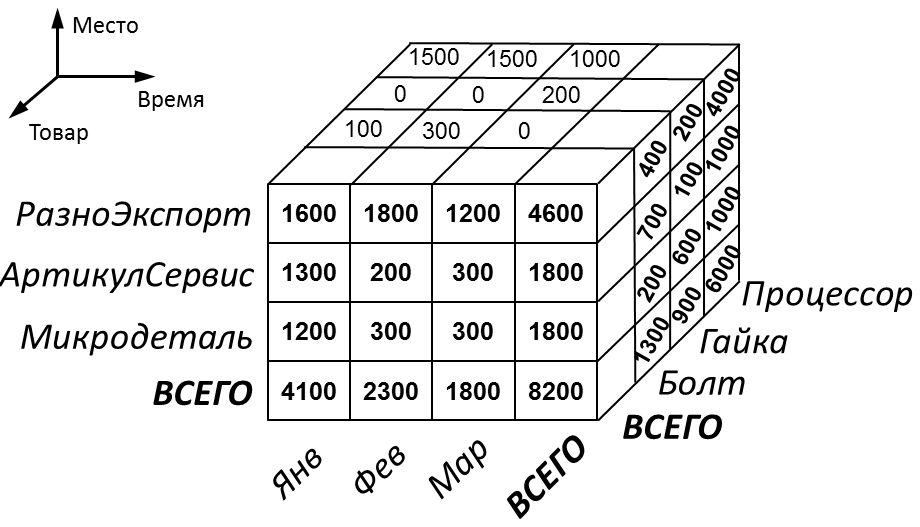
\includegraphics[scale=0.5]{olap.png}
  \caption{Пример OLAP-куба}
  \label{olap}
\end{figure}

\textit{Срез} OLAP-куба представляет собой подкуб исходного куба, полученный путем фильтрации данных по одной или нескольким осям. Пример срезов OLAP-куба модельной предметной области представлен на рис. \pic{olap-slice}.

\begin{figure}[h]
  \centering
  \begin{subfigure}[h]{\textwidth}
    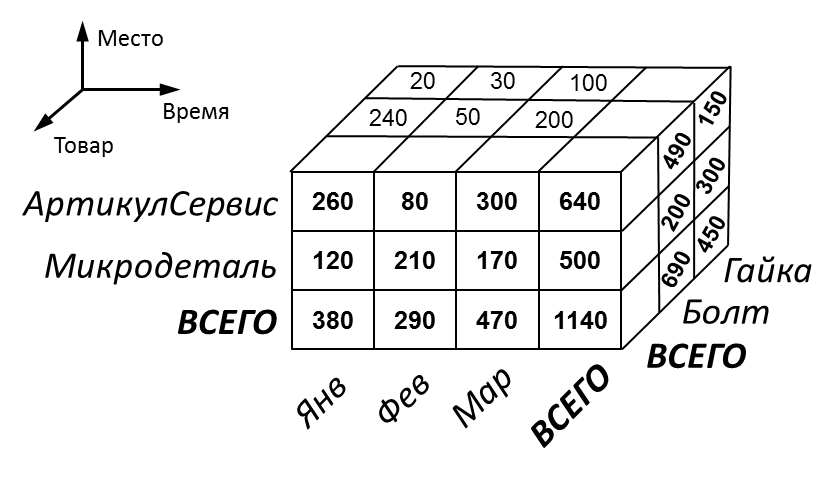
\includegraphics[scale=0.5]{olap-slice.png}
    \caption{3-мерный срез OLAP-куба}
    \label{olap-slice-3d}
  \end{subfigure} \par
  \begin{subfigure}[h]{\textwidth}
    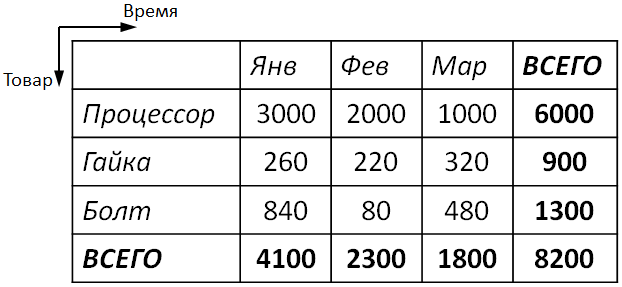
\includegraphics[scale=0.5]{olap-slice-2d.png}
    \caption{2-мерный срез OLAP-куба}
    \label{olap-slice-2d}
  \end{subfigure}
  \caption{Пример срезов OLAP-куба}
  \label{olap-slice}
\end{figure}

Визуализация OLAP-куба и его срезов предполагает возможность \textit{консолидации (roll-up)} и \textit{детализации (drill-down) данных} в соответствии с уровнями иерархии в измерениях. Пример консолидированных данных приведен на рис. \pic{consolidation}. Источником данных этих примеров являются детализированные данные среза OLAP-куба, показанного на рис. \pic{olap-slice-2d}.

\begin{figure}[h]
  \centering
  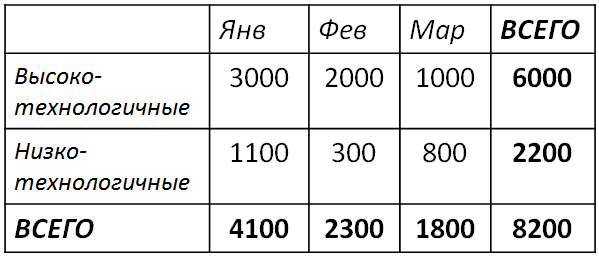
\includegraphics[scale=0.5]{consolidation.png}
  \caption{Пример консолидации данных}
  \label{consolidation}
\end{figure}

\subsubsection{Интеллектуальный анализ данных}
Система анализа бизнес-данных должна обеспечивать \textit{интеллектуальный анализ данных (Data Mining)}, который обеспечивает следующие основные функции: классификация, кластеризация и поиск шаблонов.\par
\textit{Классификация данных} предполагает автоматизированное распределение данных по непересекающимся классам, количество и семантика которых заранее известны. Классификация выполняется на основе \textit{обучающей} выборки данных, в которой классы заранее указаны экспертом.\par
Система анализа бизнес-данных должна обеспечивать интерфейс для выполнения разбиения поставщиков на три категории по риску сотрудничества с ними: низкий, средний, высокий. Для классификации поставщиков должны использоваться следующие атрибуты: общая сумма поставок от данного поставщика, общее количество поставленных данным поставщиком деталей, общее количество фактов срыва поставки данным поставщиком. Срыв поставки имеет место, если фактическая дата доставки позже, чем сумма даты заказа и срока доставки.\par
\textit{Кластеризация данных} предполагает автоматизированное распределение данных по непересекающимся кластерам, количество которых заранее известно, а семантика – заранее неизвестна. В отличие от классификации, в кластеризации не участвует эксперт и не используется обучающая выборка.\par
Система анализа бизнес-данных должна обеспечивать интерфейс для выполнения кластеризации поставок, сделанных в указанный период. Для кластеризации поставок должны использоваться следующие атрибуты: вес поставки, сумма поставки, количество деталей в поставке, название детали, город детали, признак HTP детали в поставке, цена детали в поставке. \par
\textit{Поиск шаблонов} направлен на определение наборов данных, которых повторяются с частотой, не ниже указанной. Система анализа бизнес данных должна обеспечивать интерфейс для поиска наборов деталей, которые часто доставляются совместно в один и тот же день.

\section{Проектирование}
\subsection{Схема хранилища данных}
Хранилище данных основано на СУБД MySQL. На рис. \pic{etl-diagram} изображена схема таблицы хранилища данных, связи между ними и типы связей.

\begin{figure}[h]
  \centering
  \includegraphics[scale=0.8]{etl-diagram.png}
  \caption{Сема хранилища данных}
  \label{etl-diagram}
\end{figure}

В таблице \tab{etl-suppliers} представлено описание таблицы Поставщики.
\begin{table}[h]
	\caption{\space Описание таблицы хранилища Поставщики (suppliers)}
	\label{etl-suppliers}
	\begin{tabular}{|p{0.4cm}|p{2.5cm}|p{1.5cm}|p{6.3cm}|p{3.2cm}|}
		\hline
		\textbf{№} & \textbf{Атрибут} & \textbf{Ключ} & \textbf{Семантика} & \textbf{Тип данных} \\
		\hline
		1. & id & * & Уникальный код поставщика в хранилище & INT(10) \\
		\hline
		2. & name & & Имя поставщика & VARCHAR(20) \\
		\hline
		3. & city & & Город поставщика & VARCHAR(20) \\
		\hline
		4. & address & & Адрес поставщика & VARCHAR(20) \\
		\hline
		5. & risk & & Риск поставщика & TINYINT(2) \\
		\hline
	\end{tabular}
\end{table}

В таблице \tab{etl-parts} представлено описание таблицы Детали.
\begin{table}[h]
	\caption{\space Описание таблицы хранилища Детали (details)}
	\label{etl-parts}
	\begin{tabular}{|p{0.4cm}|p{2.5cm}|p{1.5cm}|p{6.3cm}|p{3.2cm}|}
		\hline
		\textbf{№} & \textbf{Атрибут} & \textbf{Ключ} & \textbf{Семантика} & \textbf{Тип данных} \\
		\hline
		1. & id & * & Уникальный код детали в хранилище & INT (10) \\
		\hline
		2. & name & & Название детали & VARCHAR(20) \\
		\hline
		3. & HTP & & Относится ли деталь к продуктам высоких технологий & TINYINT(1) \\
		\hline
		4. & Weight & & Вес детали & FLOAT \\
		\hline
	\end{tabular}
\end{table}

В таблице \tab{etl-shipments} представлено описание таблицы Поставки.
\begin{table}[h]
	\caption{\space Описание таблицы хранилища Поставки (shipments)}
	\label{etl-shipments}
	\begin{tabular}{|p{0.4cm}|p{2.5cm}|p{1.5cm}|p{6.3cm}|p{3.2cm}|}
		\hline
		\textbf{№} & \textbf{Атрибут} & \textbf{Ключ} & \textbf{Семантика} & \textbf{Тип данных} \\
		\hline
		1. & sid & & Уникальный код поставщика в хранилище & INT(10) \\
		\hline
		2. & pid & & Уникальный код детали в хранилище & INT(10) \\
		\hline
		3. & qty & & Количество деталей в поставке & SMALLINT \\
		\hline
		4. & price & & Цена поставки & SMALLINT \\
		\hline
		5. & weight & & Вес поставки & FLOAT \\
		\hline
		6. & order\_date & & Дата заказа поставки & INT(10) \\
		\hline
		7. & period & & Время поставки & TINYINT(3) \\
		\hline
		8. & ship\_date & & Дата поставки & INT(10) \\
		\hline
	\end{tabular}
\end{table}

В таблице \tab{etl-updates} представлено описание таблицы Обновления, в которой содержится информация о том, какие данные были загружены из филлиалов.
\begin{table}[h]
	\caption{\space Описание таблицы хранилища Обновления (updates)}
	\label{etl-updates}
	\begin{tabular}{|p{0.4cm}|p{2.5cm}|p{1.5cm}|p{6.3cm}|p{3.2cm}|}
		\hline
		\textbf{№} & \textbf{Атрибут} & \textbf{Ключ} & \textbf{Семантика} & \textbf{Тип данных} \\
		\hline
		1. & time & & Время обновления & INT (10) \\
		\hline
		2. & affiliate\_id & & Номер филлиала & SMALLINT(5) \\
		\hline
		4. & S & & Последний id поставщика в филлиале affiliate\_id, который был добавлен при добавлении & INT(10) \\
		\hline
		5. & P & & Последний id детали в филлиале affiliate\_id, который был добавлен при добавлении & INT(10) \\
		\hline
		6. & SP & & Последний id поставки в филлиале affiliate\_id, который был добавлен при добавлении & INT(10) \\
		\hline
	\end{tabular}
\end{table}

\subsection{ETL}
\subsection{Функции OLAP}
\subsection{Функции интеллектуального анализа данных}
\subsection{Интерфейс пользователя}
\section{Реализация}

\end{document}